% This file was created by tikzplotlib v0.9.1.
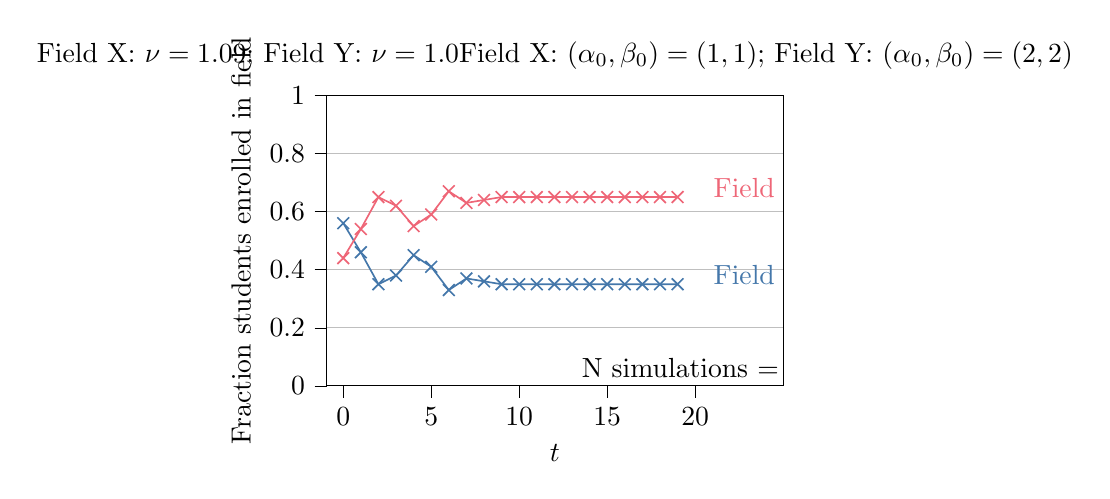
\begin{tikzpicture}

\definecolor{color0}{rgb}{0.266666666666667,0.466666666666667,0.666666666666667}
\definecolor{color1}{rgb}{0.933333333333333,0.4,0.466666666666667}

\begin{axis}[
height=150pt,
tick align=outside,
tick pos=left,
title={Field X: \(\displaystyle \nu=1.09\); Field Y: \(\displaystyle \nu=1.0\) \\ Field X: \(\displaystyle (\alpha_0, \beta_0)=(1, 1)\); Field Y: \(\displaystyle (\alpha_0, \beta_0)=(2, 2)\)},
width=210pt,
x grid style={white!69.0196078431373!black},
xlabel={\(\displaystyle t\)},
xmin=-0.95, xmax=25,
xtick style={color=black},
xtick={0,5,10,15,20},
xticklabels={\(\displaystyle 0\),\(\displaystyle 5\),\(\displaystyle 10\),\(\displaystyle 15\),\(\displaystyle 20\)},
ylabel={Fraction students enrolled in field},
ymajorgrids,
ymin=0, ymax=1,
ytick style={color=black},
ytick={0,0.2,0.4,0.6,0.8,1},
yticklabels={\(\displaystyle 0\),\(\displaystyle 0.2\),\(\displaystyle 0.4\),\(\displaystyle 0.6\),\(\displaystyle 0.8\),\(\displaystyle 1\)}
]
\addplot [semithick, color0, mark=x, mark size=3, mark options={solid}]
table {%
0 0.56
1 0.46
2 0.35
3 0.38
4 0.45
5 0.41
6 0.33
7 0.37
8 0.36
9 0.35
10 0.35
11 0.35
12 0.35
13 0.35
14 0.35
15 0.35
16 0.35
17 0.35
18 0.35
19 0.35
};
\addplot [semithick, color1, mark=x, mark size=3, mark options={solid}]
table {%
0 0.44
1 0.54
2 0.65
3 0.62
4 0.55
5 0.59
6 0.67
7 0.63
8 0.64
9 0.65
10 0.65
11 0.65
12 0.65
13 0.65
14 0.65
15 0.65
16 0.65
17 0.65
18 0.65
19 0.65
};
\draw (axis cs:20.5,0.35) node[
  anchor=base west,
  text=color0,
  rotate=0.0
]{Field X};
\draw (axis cs:20.5,0.65) node[
  anchor=base west,
  text=color1,
  rotate=0.0
]{Field Y};
\draw (axis cs:13,0.03) node[
  anchor=base west,
  text=black,
  rotate=0.0
]{N simulations = 100};
\end{axis}

\end{tikzpicture}
